\documentclass[10pt,a4paper]{article}

\usepackage{ctable}
\usepackage[T1]{fontenc}
\usepackage[utf8]{inputenc}
\usepackage{lrec2006}
%\usepackage{apacite}
\usepackage{covington}
\usepackage{tikz-qtree}

%\bibliographystyle{apacite}

\let\app=\textsc
\newcommand\deprel[1]{\\\textsc{#1}}

\tikzset{edge from parent/.style={->,draw,font={\scshape\small}},
    every tree node/.style={align=center,anchor=north},
    level distance=10ex}

\title{The Norwegian Dependency Treebank}

\name{\bf Per Erik Solberg$^{\ast}$, Arne Skj{\ae}rholt$^{\dagger}$, 
        Lilja {\O}vrelid$^{\dagger}$, Kristin Hagen$^{\ddag}$, 
        and Janne Bondi Johannessen$^{\ddag}$}%[0.2ex]
\address{         \mbox{}$^{\ast}$ Spr{\aa}kbanken, The National Library of Norway\\[0.2ex]
         \mbox{}$^{\dagger}$ Department of Informatics, University of Oslo\\[0.2ex]
        \mbox{}$^{\ddag}$ Department of Linguistics and Scandinavian Studies, University of Oslo\\
                p.e.solberg@ifikk.uio.no, $\{$arnskj,liljao$\}$@ifi.uio.no, $\{$kristin.hagen,j.b.johannessen$\}$@iln.uio.no
%
        \vspace*{1.5ex}}

%% \name{Per Erik Solberg$^{\ast}$, Arne Skj{\ae}rholt$^{\dagger}$, Lilja {\O}vrelid$^{\dagger}$, Kristin Hagen$^{\ddag}$, Janne Bondi Johannessen$^{\ddag}$}

%% \address{ Spr{\aa}kbanken, Department of Informatics, Department of Linguistics and Scandinavian Studies \\
%%                National Library, University of Oslo, University of Oslo \\
%%                author1@xxx.yy, author2@zzz.edu, author3@hhh.com\\}


\abstract{The Norwegian Dependency Treebank is a new syntactic treebank for Norwegian Bokmål and Nynorsk with manual syntactic and morphological annotation, developed at the National Library of Norway
in collaboration with the University of Oslo.
This paper presents the core principles behind the syntactic annotation and how these principles were employed in certain specific cases, the selection of texts and distribution between genres,
the annotation process and an evaluation of the inter-annotator agreement, and finally, the first results of data-driven dependency parsing of Norwegian, contrasting three state-of-the-art dependency parsers trained on the treebank. 
The consistency and the parsability of this treebank is shown to be comparable to other large treebank initiatives.  \\ \newline \Keywords{keyword A, keyword B, keyword C}}



\date{}

%\frenchspacing

\begin{document}

\maketitleabstract

\section{Introduction}
A syntactic treebank constitutes an important language resource in
establishing a set of natural language processing tools for a
language and may be employed for central tasks such as part-of-speech
tagging and syntactic parsing as well as for linguistic research. For the past decade, dependency
analysis has become an increasingly popular form of syntactic analysis
and has been claimed to strike a balance between a depth of analysis
sufficient for many down-stream applications, as well as providing accuracy and
efficiency in parsing with these types representations. The CoNLL
shared tasks devoted to dependency parsing and joint syntactic and
semantic parsing,
\cite{Niv:Hal:Kub:07,Haj:Cia:Joh:09}, have been instrumental in
establishing a common set of dependency treebanks for a range of
languages such as English, Swedish, Czech and Arabic, %% \footnote{Note
%%   that several of the treebanks employed for the shared task were not
%%   originally dependency treebanks, but rather converted from
%%   phrase-structure representations.}
thus enabling multilingual evaluation of different systems.  The increased
availability of dependency parsers has spurred down-stream use of
dependency representations in diverse tasks such as Machine Translation \cite{Din:Pal:05}, Sentiment Analysis \cite{Wil:Wie:Hof:09} and Negation Resolution \cite{Lap:Vel:Ovr:12}.

Until recently, no treebank has been available for
Norwegian.\footnote{A treebank of deep linguistic analysis couched in
  the LFG framework is however under development at the University of Bergen
  by the INESS project.}
%Hence, the progress in parsing and applications
%described above has not been possible for Norwegian.
At present, however, Spr{\aa}kbanken, at the Norwegian National Library,
is in the process of completing a two year project with the aim of
producing a dependency treebank for Norwegian.

In this paper we present the result of this project, the Norwegian
Dependency Treebank (NDT)\footnote{In the development phase, the treebank has also been referred to as Språkbanken's Gold Standard Corpus.}, a syntactic treebank which encompasses
treebanks for both variants of Norwegian (Bokm{\aa}l and
Nynorsk).\footnote{These are the two written varieties of Norwegian.}
We describe the main annotation principles employed
in the syntactic analysis of the treebank and discuss the selection of
texts. We then go on to describe the annotation process in some
detail. Finally, we present first results for data-driven dependency
parsing of Norwegian.

%312 words

\section{Annotation principles}
\subsection{General principles}

%The NDT is released in the CoNLL format, a tab-separated table consisting of the following 10 fields: token index, word form, lemma, coarse-grained part-of-speech (POS), fine-grained POS, morphological features, index of head, dependency relation and two fields which are left blank in NDT \cite{Niv:Hal:Kub:07}. 
%The texts in the NDT are lemmatized, morphologically tagged and annotated with dependency relations and head-dependent graphs. The lemmatization and morphological tagging follow quite closely the Oslo-Bergen Tagger (\cite{Joh:Hag:No:Lyn:2011};OBT), but a few adaptions have been made, notably for spelling variants which do not comply with the official norm for Bokmål and Nynorsk \cite<cf.>{Sol:2013}.

The treebank contains both morphological and syntactic annotation. The morphological annotation follows the Oslo-Bergen Tagger \cite{Hag:Joh:Nok:00,Sol:2013}.

Independent syntactic annotation guidelines for the NDT have been developed in an iterative process in the beginning of the project period by the annotators working in the project \cite{Kin:Sol:Eri:2013}. The annotation guidelines are, to a large extent, based on the Norwegian Reference Grammar \cite{Faa:Lie:Van:97}. The Dependency Grammar annotations are inspired by the choices made in comparable treebanks, in particular the Swedish treebank Talbanken \cite{Niv:Nil:Hal:2006} and the treebank of old Indo-European languages PROIEL \cite{Hau:Joh:Eck:Wel:Her:Mut:2009}.

When developing the annotation guidelines, four fundamental principles were taken into consideration:
\begin{enumerate}
 \item \textbf{Linguistic adequacy:} The annotation should be as linguistically adequate as possible.
 \item \textbf{Consistency:} It had to be possible for annotators to implement the analyses consistently.
 \item \textbf{Quick annotation:} As size matters for most users, the annotators should be able to annotate quickly.
 \item \textbf{Easy retrieval:} It should be easy to retrieve specific constructions.
\end{enumerate}
In what remains of this section, we will show examples of how we tried to implement these principles, and compare our choices to other annotation schemes.

\subsection{Adverbials}
In some treebanks comparable to the NDT, e.g. Talbanken, there are separate dependency relations for different types of adverbials, such as time adverbials, manner adverbials and place adverbials. 
% Some treebanks, e.g. PROIEL \cite{Hau:Joh:Eck:Wel:Her:Mut:2009}, distinguish between adverbials selected by specific predicates, such as motion verbs, and adverbial modifiers which are not obligatory.
%There may be good linguistic reasons for making such distinctions. However, w
We found that it would be difficult to have such distinctions and at the same time comply with the consistency and time constraints of principle 2 and 3. %, as there would be frequent borderline cases.
%Unless the guidelines contained rules which were clear and easy to follow for such cases, chances are high that an annotator would not be able to annotate similar cases in a uniform manner, and inter-annotator consistency would also be difficult to obtain. And even with such rules in place, annotators would spend a considerable amount of time deliberating which dependency relation to choose. As adverbials are highly frequent and the time frame of the project was rather small, a fine-grained analysis of adverbials would have had a non-negligible impact on the size of the corpus.
When making annotation choices, we also opted for analyses which are meaningful to various end user groups.
In this light, a high level of linguistic detail is not always an advantage, as it becomes more difficult to infer grammatical patterns and extract meaningful information \cite{Mar:Man:08}.
A fine-grained analysis of adverbials could in fact make such tasks more difficult, as distinctions between different types of adverbials frequently would be based on semantic and pragmatic considerations only, not on difference in syntactic structure.
For example, the same preposition may express different types of adverbials in very similar contexts, as the following pair of sentences shows:

\begin{examples}
\item\label{ex:locadv}
\gll Per jobber på en skole.
Per works on a school
\glt `Per works at a school.'
\glend

\item\label{ex:timeadv}
\gll Per jobber på en mandag.
Per works on a Monday
\glt `Per works on a Monday.'
\glend
\end{examples}

We therefore opted for a more shallow analysis:
All adverbials, regardless of type,
and of whether or not they are selected,
receive a uniform dependency relation - ADV. 

\subsection{Transitive and intransitive prepositions}
In other cases, the pursuit of linguistic adequacy (principle 1) has been given priority. The sentences (\ref{ex:intrans}) and (\ref{ex:trans}) exemplify such a case:

\begin{examples}
\item\label{ex:intrans}
\gll Per setter på CD-en.
Per puts on CD+the
\glt `Per puts on the CD.'
\glend

\item\label{ex:trans}
\gll Per sitter på stolen.
Per sits on chair+the
\glt `Per sits on the chair.'
\glend
\end{examples}

In both (\ref{ex:intrans}) and (\ref{ex:trans}), the preposition \emph{på} is followed by a noun. There are, however, strong reasons for analyzing the sentences differently. In (\ref{ex:trans}), the noun is clearly a complement of the preposition: The preposition and the noun are semantically connected, they behave as a single constituent, and the complement retains its position after the preposition if it is pronominalized. In (\ref{ex:intrans}), there is no obvious semantic connection between the preposition and the noun, the two words do not form a constituent together, and if the noun is pronominalized, it usually will precede the preposition. In the NDT, the noun in constructions like (\ref{ex:intrans}) would be made dependent on the verb with the dependency relation for direct objects, DOBJ, while in (\ref{ex:trans}), it is made dependent on the preposition with the dependency relation of prepositional complements, PUTFYLL.

Annotators frequently meet preposition-noun sequences which are less straightforward than in these examples, and they need to deliberate whether one or the other analysis is correct. We have, however, chosen to retain this distinction, to make sure that the analyses are acceptable from a linguistic point of view and also in order to achieve a uniform analysis of sentences such as (\ref{ex:intrans}) and cases where the object noun or pronoun does not follow the intransitive preposition (or particle, as these are also known). To ensure consistency and a high annotation speed (principle 2 and 3), the annotation guidelines have a number of syntactic tests which the annotators use to distinguish between the constructions \cite[54-56]{Kin:Sol:Eri:2013}.

\subsection{Complementizers}
There is no obvious head-dependent relationship between complementizers and verbs or between lexical and function words in general, and there is therefore not a unique answer to how such a relationship should be represented in Dependency Grammar.
In the original formulation of Dependency Grammar, no dependency relations were indicated between function words and lexical words. Instead, a different, symmetrical relation was used \cite[361-410]{Tes:65}. 
In Dependency Grammar treebanks comparable to the NDT, no relations apart from assymetrical dependency relations are used.
This makes the annotations easy to represent too humans and to process for standard software \cite[4]{Mar:Man:08}.
Some annotation standards treat all relations between lexical and functional words in the same manner. In the Standford annotation standard, the lexical word is the head whenever possible \cite[2]{Mar:Man:08}.
In NDT, we have no uniform treatment of lexical and function words, but we have made a decision for each construction, based on the four principles given above. For example, in the case of complementizers and verbs, we have chosen to let the verb be the head and the complementizer a dependent on the verb. The reason for this is that
%Treebanks vary with respect to the annotation of the complementizer-verbs relations and similar relations between functional and lexical heads.
%In the NDT, the verb is the head and the complementizer is a dependent on the verb. This choice is first and foremost motivated by the fourth principle stated above: easy querying.
complementizers are frequently dropped in Norwegian, as the following examples show (from the NDT):

\begin{examples}
\item\label{ex:medat}
\gll Nå tror lokale myndigheter at bortføringen var nøye planlagt.
now believe local authorities that.comp abduction+the was carefully planned
\glt `Local authorities now believe that the abduction was carefully planned.'
\glend

\item\label{ex:utenat}
\gll Jeg tror ikke det er tilfeldig.
I believe not it is accidental
\glt `I don't belive that it is accidental.'
\glend
\end{examples}

Clausal complements of verbs such as \emph{tro}, 'believe', occur both with the complementizer \emph{at}, as in (\ref{ex:medat}), and without any complementizer, as in (\ref{ex:utenat}). If the complementizer were the head, the complement clauses in (\ref{ex:medat}) and (\ref{ex:utenat}) would have had different heads, despite their obvious similarities. This, in turn, would make it significantly more difficult to formulate queries using standard query tools, and more difficult to deduce grammatical patterns more generally (cf. principle 4).
%The ability to retrieve constructions through queries has been important in the annotation process, notably in order to find annotation errors, and it will probably also be important to certain users of the treebank.
In the NDT,
sentences such as (\ref{ex:medat}) and (\ref{ex:utenat}) are analyzed similarly: The (finite) verb of the clausal complement serves as head in both cases, and carries the dependency relation DOBJ (direct object), c.f. figure \ref{figure:medat} and \ref{figure:utenat}.
Both will therefore be retrieved through a query for finite verbs with the dependency relation DOBJ.

\subsection{Other choices of analysis}
Table \ref{tb:choices} summarizes some choices where dependency treebanks tend to differ. The coordination analysis follows \newcite{Niv:Nil:Hal:2006}:
The first conjunct is the head and carries the grammatical function of the whole coordinated structure. Subsequent conjuncts are dependent on the first with the function KOORD.
Conjunctions are dependent on the closest conjunct to the right and receive the function KONJ.

We have chosen to let the finite verb always be the head of a finite clause. As a consequence of this, a finite auxiliary, when present, will be head, taking the lexical verb as its dependent with the function INFV.
Subjects will be dependents on the finite verb, while other arguments will attach to the lexical verb.

Determiners are dependents on nouns in NDT, with the function DET.

The analysis in figure (\ref{figure:koord}) of sentence (\ref{ex:koord}) exemplifies the annotation choices mentioned in this subsection.

\begin{examples}
\item\label{ex:koord}
\gll Per har spist et eple og en pære
Per has eaten an apple and a pear
\glt `Per has eaten an apple and a pear.'
\glend
\end{examples}


\ctable[botcap,
    caption={Annotation choices in the NDT},
    label=tb:choices,
]{ll}{}{
        \FL
\multicolumn{1}{c@{\hspace{1em}}}{Head} & \multicolumn{1}{c@{\hspace{0.5em}}}{Dependent} \ML
Preposition & Prepositional complement \NN
Finite verb & Complementizer \NN
First conjunct & Subsequent conjuncts \NN
Finite auxiliary & lexical/main verb \NN
Noun & Determiner
        \LL
    }

\begin{figure}
    \begin{center}
        %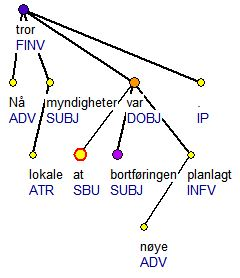
\includegraphics{medat.jpg}
        \Tree [.tror\deprel{FINV}
                Nå\deprel{ADV}
                [.myndigheter\deprel{SUBJ}
                    lokale\deprel{ATR} ]
                [.var\deprel{DOBJ}
                    at\deprel{SBU}
                    bortføringen\deprel{SUBJ}
                    [.planlagt\deprel{infv} nøye\deprel{ADV} ] ]
                {\vphantom{I}.}\deprel{IP} ]
    \end{center}
    \caption{Analysis of (\ref{ex:medat})}
    \label{figure:medat}
\end{figure}

\begin{figure}
    \begin{center}
        %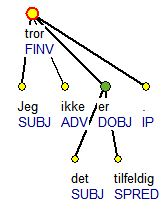
\includegraphics{utenat.jpg}
        \Tree [.tror\deprel{FINV}
                jeg\deprel{SUBJ}
                ikke\deprel{ADV}
                [.er\deprel{DOBJ}
                    det\deprel{SUBJ}
                    tilfeldig\deprel{SPRED} ]
                {.}\deprel{IP} ]
    \end{center}
    \caption{Analysis of (\ref{ex:utenat})}
    \label{figure:utenat}
\end{figure}

\begin{figure}
    \begin{center}
        \Tree [.har\deprel{FINV}
                Per\deprel{SUBJ}
                [.spist\deprel{INFV}
                [.eple\deprel{DOBJ}
                    et\deprel{DET}
                   [. pære\deprel{KOORD}
                      og\deprel{KONJ} 
                      en\deprel{DET}  ] ] ]
                {.}\deprel{IP} ]
    \end{center}
    \caption{Analysis of (\ref{ex:koord})}
    \label{figure:koord}
\end{figure}


\section{Texts}
The NDT consist of 311 000 tokens of Norwegian Bokmål and 303 000 tokens of Norwegian Nynorsk. The texts for Bokmål and Nynorsk were collected from independent sources. Since the differences between these two written standards of Norwegian are mostly lexical and morphological, the syntactic annotation is practically identical. Comparable treebanks such as the Prague Dependency Treebank and the TIGER treebank, contain mainly newspaper text \cite{Boh:Haj:Hla:2003,Bra:2004}. Other treebanks, e.g. Penn Treebank and Talbanken \cite{Mar:San:Mar:93,Niv:Nil:Hal:2006}, however, also contain texts from other sources, such as factual prose, fiction and text in a more colloquial style.

Newspaper text is frequently used for various NLP tasks and also has the advantage of being fairly standardized, unlike fiction and e.g. texts from social media. We have therefore chosen to use mostly newspaper text in the NDT, but we added small amounts of text from government reports, parliament transcripts and more colloquial texts from blogs, cf. table \ref{tb:distribution}.
%In the final version of the NDT, it will be possible to extract specific genres of text.

\ctable[botcap,
    caption={Distribution of texts in the treebanks},
    label=tb:distribution,
    mincapwidth=\columnwidth
]{lr@{\%\hspace{0.5em}}}{}{
        \FL
        Source & \multicolumn{1}{c}{Fraction} \ML
Newspaper text & 82 \NN
Government reports & 7 \NN
Parliament transcripts & 6 \NN
Blogs & 5
        \LL
    }

% 138 words 

\section{Annotation process}
\subsection{Annotators}
All texts in the treebank have been manually annotated by trained linguists. A
few of the texts have been syntactically annotated by two annotators, to
avoid inconsistencies (cf. \ref{sc:inter-a}). In order to speed up the annotation
process, we chose to preprocess the texts using tools already available at the
University of Oslo.

\subsection{Preprocessing and work flow}
As is standard practice when annotating syntactic corpora, the texts to be
annotated are automatically PoS tagged and syntactically parsed before being
annotated, an approach which has been shown to be both fast and yielding
high quality annotation \cite{Mar:San:Mar:93,For:Sag:10,Skjaerholt:13}.
After tokenization, the texts are first tagged using OBT+stat,
a rule-based Constraint Grammar tagger with a HMM-based overlay \cite{Johannessen:etal:12}.
 The morphological annotation is then checked and corrected by an annotator using a web interface made for this
particular task \cite{Lyn:13}. The corrected morphological annotations are
then preprocessed by a dependency parser and imported into \app{TrEd}, the
annotation tool developed for the Prague Dependency Treebank, which is used to
correct the output of the syntactic preprocessing and create the final
treebank.

%Since there were no publicly available dependency corpora at the start of this
%project, training a data-driven dependency parser was
%impossible. Therefore, t
The initial syntactic preprocessor was created using
the syntactic module of OBT, which, while it does not create a hierarchical
structure, does provide some information about heads. On top of this we built
a small set of rules in the CG-3 framework \cite{Did:2013} to build proper
syntactic structures. This preprocessor was evaluated to get about 80\% of
heads correct (unlabeled attachment) and both head and label (labeled
attachment) correct in 72--74\% of cases, as shown in Table \ref{tbl:parsers}.

The first statistical parser trained on the corpus is that of
\newcite{Skj:Ovr:12}, which was later used in inter-annotator agreement
experiments by \newcite{Skjaerholt:13}, reported to reach a labeled accuracy of
84\% and an unlabeled accuracy of 87\%. Based on this, an improved parser was
trained which obtains an unlabeled accuracy of nearly 90\% and labeled
accuracy of 87\%.
%Note that these results are not entirely comparable as they
%are evaluated on different corpora, but given the important differences in
%performance, the improved parsers are clearly better. In particular, the
%difference between the CG parser and that of \citeA{Skj:Ovr:12} resulted in
%significant increases in annotator productivity \cite{Skjaerholt:13}.

\ctable[botcap,
    caption={Preprocessor accuracies. Unlabeled (UAS) and Labeled (LAS)
    attachment scores, and label accuracies (Labels).},
    label=tbl:parsers,
    mincapwidth=\columnwidth,
    notespar,
]{l@{~(}c@{)\hspace{1em}}r@{.}lr@{.}lr@{.}l}{}{
        \FL
\multicolumn{2}{c}{Parser} & \multicolumn{2}{c@{\hspace{1em}}}{UAS} & \multicolumn{2}{c@{\hspace{1em}}}{LAS} & \multicolumn{2}{c@{\hspace{0.5em}}}{Labels} \ML
CG & BM            & 79&39\% & 72&45\% & 82&10\% \NN
CG & NN            & 80&16\% & 74&76\% & 84&84\% \NN
S \& Ø (2012) & BM & 87&54\% & 84&63\% & 89&63\% \NN
Final & BM         & 89&89\% & 87&57\% & 91&70\% \NN
Final & NN         & 89&66\% & 87&50\% & 91&76\%
        \LL
    }

% Need to set a standard evaluation corpus to properly compare the different
% preprocessors. Which has to be different from the training material of *all*
% the MaltParsers (most important in that respect is the most recent one from
% PE.
%
% Given this, it might make sense to merge or at least connect this part to
% the section of dependency parsing.

\subsection{Inter-annotator agreement}
\label{sc:inter-a}
To validate the consistency of the annotations produced by the different
annotators, a set of experiments quantifying inter-annotator agreement were
performed \cite{Skjaerholt:13}. As is common practice in the field of
syntactic annotation \cite{Civit:ea:03,Brants:00,Bra:Han:02,Hajic:04}, the
simple agreement measures labeled and unlabeled attachment accuracy were
used. The reason for using an uncorrected measure rather than a
chance-corrected measure such as $\kappa$ or $\pi$ is that these measures are
not directly applicable to the task of syntactic annotation.

\newcite{Skjaerholt:13} measured inter-annotator agreement as measured by
labeled and unlabeled attachment, using a number of different preprocessors
from the cross lingual parsers of \newcite{Skj:Ovr:12}. Here, we will
concentrate on the agreement using the best parser, whose performance is shown
in Table \ref{tbl:parsers}. Using this parser, agreement was measured to be
96.8\% unlabeled and 95.3\% labeled accuracy. These results are comparable
to those reported for the German NEGRA (92.4\% labeled
$F_1$ \cite{Brants:00}) and TIGER (93.9\% labeled $F_1$ \cite{Bra:Han:02})
treebanks and the Spanish Cat3LB treebank (86.9\% labeled bracket
precision \cite{Civit:ea:03}).

A further set of experiments have been performed by \newcite{Skjaerholt:14},
quantifying agreement using a chance-corrected metric derived from
Krippendorff's $\alpha$ \cite{Krippendorff:12}. In these experiments,
agreement on the NDT data is extremely high: scoring an $\alpha$ of about
98\%, among the highest of all the data sets studied.

\section{Dependency parsing}
%TO-DO: note that final version of the paper will contain results from the final version of the treebank
An important aspect of treebank annotation relates to its \emph{parsability},
i.e. the quality of syntactic parsers that can be acquired based on
the treebank data.  In order to investigate the parser quality we can
expect from the NDT, we have evaluated three state-of-the-art dependency
parsers on the material: Maltparser \cite{Niv:Hal:Nil:06},
MST-parser \cite{McD:Per:Rib:Haj:05} and the parser of
\newcite{Boh:Niv:12}. These implement different parsing strategies: Maltparser is a transition-based parser with local learning and greedy search, MST is a graph-based dependency parser implementing global, near-exhaustive search and the \newcite{Boh:Niv:12} parser is a transition-based dependency parser with joint tagger that
implements global learning and a beam search for non-projective labeled
dependency parsing. 
This latter parser has recently outperformed pipeline systems (such as the
Malt and MST parsers).
%both in terms of tagging and parsing accuracy for
%typologically diverse languages such as Chinese, English, and German. 
For Maltparser, we trained two versions of the
parser: one version with default settings and one optimized version,
where the parser settings was optimized using the MaltOptimizer
software \cite{Bal:Niv:12}. Both the MST and \newcite{Boh:Niv:12}
parsers were trained using default settings.

For these experiments, both portions of the treebank (Bokm{\aa}l and
Nynorsk) were split into 80-10-10 train, development and test sets.
%Standard evaluation metrics in dependency parsing are unlabeled and
%labeled attachment scores (UAS, LAS; implemented by the CoNLL
%\textsf{eval.pl} scorer).  These measure the proportion of tokens
%which are correctly attached to their head token and, for LAS,
%furthermore have been assigned the correct dependency label.


%121 words


\ctable[botcap,
    caption={Dependency parsing results for the NDT},
    label=tb:parsing
]{lll@{\hspace{2em}}ll}{}{
        \FL
    & \multicolumn{2}{c@{\hspace{2em}}}{Bokm{\aa}l (BM)} & \multicolumn{2}{c}{Nynorsk (NN)} \NN
    & UAS & LAS  & UAS & LAS \ML
Malt default & 88.27 & 85.03 & 87.54 & 83.82 \NN
Malt optimized & 92.19 & 89.82 & 91.57 & 88.98 \NN
MST  & 91.69 & 88.26 & 91.54 & 87.80 \NN
Bohnet\&Nivre & 92.94 & 90.56 & 92.78 & 90.18 
        \LL
    }

Table \ref{tb:parsing} presents the dependency parsing results
obtained for the NDT. We find that the \newcite{Boh:Niv:12} parser
outperforms the other parsers and obtains labeled accuracy scores of
90.6 and 90.2 for the BM and NN treebanks, respectively.  The
optimized Maltparser model performs only slightly lower, at 89.8 and
89.0.  These are encouraging results which indicate that the treebank
provides a good basis for parser development.

\section{Conclusion}
We have presented the first treebank for Norwegian, a treebank
containing dependency representations for a large sample of Norwegian
texts
%(in both of the written standards).
We have described the
annotation principles that motivate the analyses, the collections of
texts, as well as the annotation process and presented results for
inter-annotator agreement, showing that the syntactic annotation is of
a consistency comparable to other large treebank initiatives. Finally,
we have presented the first results for Norwegian dependency parsing,
contrasting three state-of-the-art data-driven dependency parsers.

\section{Acknowledgements}

Place all acknowledgements (including those concerning research grants and funding) in a separate section at the end of the article.

%\section{References}


%\clearpage
\bibliographystyle{lrec2006}
\bibliography{ndt}

\end{document}
